\chapter{Introduction}

Here we review some of the terminologies that frequently appear in the field of Reinforcement Learning.
\section{Important Concepts}
Imagine a \textbf{discrete-time} system (environment), meaning that the system is discretized into time steps. At time step $t$, we define the state of the system to be $s_t$. The state of a system/agent could be some intrinsic data of it. For example, for a car, the state of a car at a given time step could be the car's angular velocity, acceleration, and mass. We also define an agent's action $a_t$, which is equivalent to control theory's input. A \textbf{policy} is a function that takes in a state and outputs an action, determining what the agent should do given current time step's state. 

A policy function could be deterministic such that $a_t = \pi_\theta(s_t)$. The policy function could also be a distribution, which we can define as $\pi_\theta(a_t|s_t)$. Note that in many cases, a state is not \textbf{fully observable}, so we might only partially observe the state of the agent via an observation $o_t$. In this case, the policy function should condition on the observation $o_t$. 

We should also define a \textbf{transition function} of the environment. In the most general case, the transition should be stochastic, meaning that a state could evolve into a number of other states potentially. Therefore, this function should be a distribution, defined as $p(s_{t+1}|s_t, a_t)$. Note that this distribution is conditioned on both the state and the action at time step $t$. If you are familiar with control theory, you would probably notice the resemblance of the transition distribution with a discrete-time system's dynamics function. A sequence of states and actions become a \textbf{trajectory}, which we call $\tau$.

Meanwhile, we also define a \textbf{reward function} of the environment. For example, in Pacman, the player gains one point after eating a dot, and loses 100 points after being eaten by a ghost. Formally, the reward function should be a function of both state and action, so we denote the reward function as $r(s,a)$.

In reinforcement learning, we assume the states transitions are \textbf{Markovian}, meaning that the state at time step $t$ is only responsible for contributing to the state at time step $t+1$.
Here is an illustration of a Markov chain, and the direction of the arrow means causality:
\begin{figure}
    \centering
    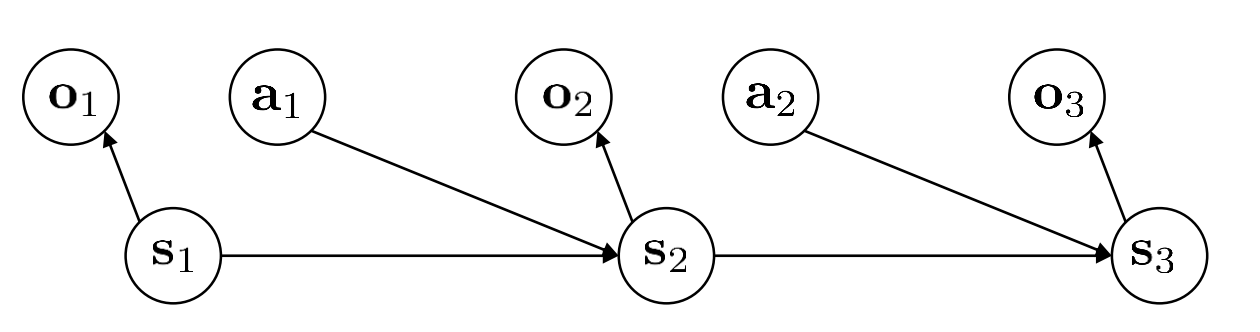
\includegraphics[scale = 0.4]{figures/markov.png}
    \caption{A simple Markov chain.}
    \label{fig:markov}
\end{figure}

In control theory, such as the LQR optimization problem, we aim to minimize the cost function of the system. What would be an equivalent notion in reinforcement learning? Recall we defined a reward function, $r(s,a)$, so naturally we want to collect as much reward as possible in the environment. Without loss of genrality, we assume that the environment is stochastic. Define a trajectory distribution $p_\theta(\tau)$ according to Baye's Rule:
$$ p(\tau) \vcentcolon= p(s_1,a_1,...,s_T,a_T) = p(s_1)\prod_{t=1}^T\pi_\theta(a_t|s_t)p(s_{t+1}|s_t,a_t)$$
where $T$ is the length of episode horizon. Therefore, given this trajectory distribution, we can calculate the expected value of the total reward function induced by following this trajectory as $\mathbb{E}_{\tau\sim p_\theta(\tau)}\left[\sum_t r(s_t,a_t)\right]$. Therefore, to optimize this objective, we want to find a parameter $\theta$, such that $\theta$ maximizes the above expectation:
$$\theta = \argminA_\theta\mathbb{E}_{\tau\sim p_\theta(\tau)}\left[\sum_t r(s_t,a_t)\right]$$
\section{Value Function and Q Function}
To facilitate our calculation of the above expectation, and to simplify the notations, we introduce two important types of functions: Q function and value function. In most cases these two functions are not given to us in closed form, and one needs to approximate and improve the functions using some deep neural net, hence the notion of ``deep'' in deep reinforcement learning.
\subsection{Q Function}
Q function is a function of both state and action, so it is denoted as $Q(s_t,a_t)$ and it quantitatively measures the quality of taking action $a_t$ at state $s_t$. Mathematically, it is the expected sum of reward from the current time step given state $s_t$ and action $a_t$. This is very similar to the ``cost-to-go'' function in control theory, especially Model Predictive Control. We define $Q(s,a)$ as:
$$Q^\pi(s_t,a_t) = \sum_{t'=t}^T{\mathbb{E}_{\pi_\theta}[r(s_t',a_t')|s_t,a_t]}$$
\subsection{Value Function}
Unlike the Q function, value function is only a function of state, so intuitively it quantitatively measures the value of being in state $s_t$. Mathematically, it is defined as $V^\pi(s_t) =\sum_{t'=t}^T{\mathbb{E}_{\pi_\theta}[r(s_t',a_t')|s_t]}$. Again by Baye's rule we can obtain the relation between Value function and Q function: $V^\pi(s_t)=\mathbb{E}_{a_t\sim\pi(a_t|s_t)}[Q^\pi(s_t,a_t)]$.

Furthermore, if we sum the value function over all possible initial states, we essentially recovered the objective of reinforcement learning: $\mathbb{E}_{s_1\sim p(s_1)[V^\pi(s_1)]}$, where $p(s_1)$ is a known distribution of all possible initial states.
\section{Reinforcement Learning Anatomy}
In RL, we usually have three parts in the whole pipeline. We need to keep generating data for the agent to learn, and use the data to generate samples in order to fit and regress onto a model. Then with this model, we estimate the reward and based on the reward we update our policy to maximize the reward, and we go back to step 1. Therefore, our primal concern is to efficiently run the three parts so that the agent can learn optimally with less data and computation. Here is an illustration of the three steps in Fig. \ref{fig:rlanatomy}.
\begin{figure}
    \centering
    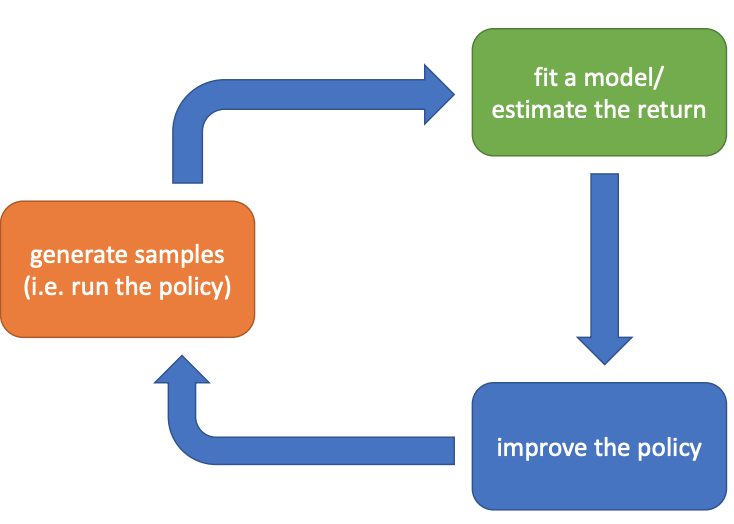
\includegraphics[scale=0.5]{figures/rlanatomy.png}
    \caption{Three steps of reinforcement learning.}
    \label{fig:rlanatomy}
\end{figure}